\hyperdef{}{tilda}{}

\subsection{Computergestützter Sprachvergleich mit Python und
JavaScript}

\begin{center}\rule{0.5\linewidth}{\linethickness}\end{center}

\subsubsection{Sitzung 2 (Tag 4)}

\begin{center}\rule{0.5\linewidth}{\linethickness}\end{center}

\paragraph{23.07.2015}

\begin{center}\rule{0.5\linewidth}{\linethickness}\end{center}

\subsubsection{\texorpdfstring{``Automatischer Sprachvergleich mit
Python''}{Automatischer Sprachvergleich mit Python}}

\subsection{\texorpdfstring{{Agenda 2015}}{Agenda 2015}}

\begin{itemize}
\itemsep1pt\parskip0pt\parsep0pt
\item
  {Automatischer Sprachvergleich}

  \begin{itemize}
  \itemsep1pt\parskip0pt\parsep0pt
  \item
    {Sequenzdistanzen}
  \item
    {Kognatenerkennung}
  \item
    {Phylogenetische Rekonstruktion}
  \end{itemize}
\item
  {Sprachvergleich mit LingPy}

  \begin{itemize}
  \itemsep1pt\parskip0pt\parsep0pt
  \item
    {Eingabeformate}
  \item
    {Analysen}
  \item
    {Ausgabeformate}
  \end{itemize}
\item
  {Workflows}

  \begin{itemize}
  \itemsep1pt\parskip0pt\parsep0pt
  \item
    {Allgemeines vorweg}
  \item
    {Kognatenerkennung mit LingPy}
  \item
    {Integration mit externen Tools}
  \end{itemize}
\end{itemize}

\subsection{\texorpdfstring{{Automatischer
Sprachvergleich}}{Automatischer Sprachvergleich}}

\subsubsection{\texorpdfstring{{Sequenzdistanzen}}{Sequenzdistanzen}}

\textbf{Von Alinierungen zu Distanzwerten}

Wenn man Sequenzen (Wörter im Falle der Linguistik) aliniert hat, dann
kann man auch ihre Distanz zueinander berechnen. Die ist implizit ja
bereits ein Teil der Berechnung der Alinierung, und sie kann
entsprechend auch einfach weiterverwendet werden, wobei man vorsichtig
sein sollte, was die Aussage einer solchen Distanz betrifft.

\subsection{\texorpdfstring{{Automatischer
Sprachvergleich}}{Automatischer Sprachvergleich}}

\subsubsection{\texorpdfstring{{Sequenzdistanzen}}{Sequenzdistanzen}}

\textbf{Die normalisierte Levenshtein-Distanz}

Eine der bekanntesten und am häufigsten verwendeten Distanzen zwischen
Strings ist die \emph{Levenshtein-Distanz}, die grundlegend die Anzahl
der \emph{Editier-Schritte} beschreibt, die notwendig sind, um eine
Sequenz in die andere zu überführen. Um eine bessere Vergleichbarkeit zu
gewährleisten, wird häufig neben der normalen
\emph{Levenshtein-Distanz}, die ein ganzzahliger Wert ist, auch die
``normalisierte Levenshtein-Distanz'' berechnet, bei der man die
``normale'' Distanz durch die Länge des größeren Strings teilt.

\subsection{\texorpdfstring{{Automatischer
Sprachvergleich}}{Automatischer Sprachvergleich}}

\subsubsection{\texorpdfstring{{Sequenzdistanzen}}{Sequenzdistanzen}}

\textbf{Die normalisierte Levenshtein-Distanz}

\begin{verbatim}
>>> from lingpy import *
>>> seqA = 'levensthein'
>>> seqB = 'levenschtein'
>>> d = edit_dist(seqA,seqB)
>>> d
1
>>> def norm_ed(a,b):
...     return edit_dist(a,b) / max(len(a), len(b))
...
>>> norm_ed(seqA, seqB)
0.08333333333333333
>>> edit_dist(seqA, seqB, normalized=True)
0.08333333333333333
\end{verbatim}

\subsection{\texorpdfstring{{Automatischer
Sprachvergleich}}{Automatischer Sprachvergleich}}

\subsubsection{\texorpdfstring{{Kognatenerkennung}}{Kognatenerkennung}}

\textbf{Automatisches Erkennen von kognaten Wörtern}

Kognaten sind, daran sei noch mal erinnert, Wörter, die auf einen
gemeinsamen Vorgänger zurückgehen (wie bspw. Deutsch \emph{Hand} und
English \emph{hand}). Automatisch können wir eine recht einfache
Heuristik entwickeln, um festzustellen, ob zwei Wörter kognat sind (was
nicht heißt, dass sie das auch wirklich sind!). Wir können einfach
sagen, dass, wenn immer zwei Wörter sich mehr ähneln als gewöhnlich, wir
annehmen, dass diese kognat sind. Die Ähnlichkeit können wir dabei
natürlich unterschiedlich definieren!

\subsection{\texorpdfstring{{Automatischer
Sprachvergleich}}{Automatischer Sprachvergleich}}

\subsubsection{\texorpdfstring{{Kognatenerkennung}}{Kognatenerkennung}}

\textbf{Die Lautklassenheuristik}

Eine erste einfache Heuristik besagt, dass zwei Wörter immer dann als
kognat klassifiziert werden, wenn sie in den ersten beiden Lautklassen,
die Konsonanten sind, übereinstimmen
(\href{http://bibliography.lingpy.org?key=Turchin2010}{Turchin et al.
2010}).

\begin{verbatim}
>>> seqA = sampa2uni('Tri')
>>> seqB = sampa2uni('drai')
>>> seqA, seqB 
('θri', 'drai')
>>> clsA = tokens2class(ipa2tokens(seqA), 'dolgo')
>>> clsB = tokens2class(ipa2tokens(seqB), 'dolgo')
>>> clsA = ''.join(clsA).replace('V','')
>>> clsB = ''.join(clsB).replace('V','')
>>> clsA[:2] == clsB[:2]
True
>>> clsA, clsB
('TR', 'TR')
>>> turchin(seqA, seqB)
0
>>> turchin(seqA, 'test')
1
\end{verbatim}

\subsection{\texorpdfstring{{Automatischer
Sprachvergleich}}{Automatischer Sprachvergleich}}

\subsubsection{\texorpdfstring{{Kognatenerkennung}}{Kognatenerkennung}}

\textbf{Schwellenwerte}

Anstelle des Kriteriums von
\href{http://bibliography.lingpy.org?key=Turchin2010}{Turchin et al.
(2010)} könnenwir natürlich auch andere Verfahren verwenden. Zum
Beispiel können wir sagen, dass ab einem bestimmten Schwellenwert der
normalisierten Levenshtein-Distanz zwei Wörter nicht mehr kognat sind:

\begin{verbatim}
>>> def cognate(seqA, seqB, threshold=0.4):
...     if edit_dist(seqA, seqB, normalized=True) > threshold:
...         return 1
...     return 0
... 
>>> seqA = sampa2uni('t_hOxt@r')
>>> seqB = 
KeyboardInterrupt
>>> seqA = sampa2uni('t_hOxt_h@r')
>>> seqB = sampa2uni('dO:t_h@r')
>>> cognate(seqA, seqB)
\end{verbatim}

\subsection{\texorpdfstring{{Automatischer
Sprachvergleich}}{Automatischer Sprachvergleich}}

\subsubsection{\texorpdfstring{{Phylogenetische
Rekonstruktion}}{Phylogenetische Rekonstruktion}}

\textbf{Von Distanzen zu Bäumen}

Wenn wir ermittelt haben, welche Wörter in welchen Sprachen miteinander
kognat sind, können wir Distanzen zwischen ganzen Sprachen berechnen.
Dazu zählen wir einfach alle kognaten Wörter in unserem Sample und
teilen dann die Anzahl der kognaten Wörter durch die Gesamt-Anzahl der
Wörter und ziehen diesen Wert von 1 ab (ansonsten hätten wir eine
Ähnlichkeit und keine Distanzen).

\subsection{\texorpdfstring{{Automatischer
Sprachvergleich}}{Automatischer Sprachvergleich}}

\subsubsection{\texorpdfstring{{Phylogenetische
Rekonstruktion}}{Phylogenetische Rekonstruktion}}

\textbf{Kleines Beispiel zur Distanzberechnung}

\begin{verbatim}
from lingpy import *
# die daten
data = dict(
    german = ['hant', 'fuːs', 'kɔp͡f'],
    english = ['hænd', 'fʊt', 'hɛd'],
    dutch = ['hant', 'vut', 'kɔp']
    )
# die sprachen
taxa = ['german', 'english', 'dutch']
# die distanzmatrix
matrix = [[0 for i in range(3)] for j in range(3)]
for i,k in enumerate(taxa):
    for j,l in enumerate(taxa):
        # wir müssen nur ein mal pro sprachpaar vergleichen
        if i < j:
            score = 0
            for seqA, seqB in zip(data[k], data[l]):
                score += edit_dist(seqA, seqB, normalized=True)
            score = score / 3
            matrix[i][j] = score
            matrix[j][i] = score
# der baum
tree = upgma(matrix, taxa)
# ascii-art mit Hilfe von LingPy
print(Tree(tree).asciiArt())
\end{verbatim}

\subsection{\texorpdfstring{{Automatischer
Sprachvergleich}}{Automatischer Sprachvergleich}}

\subsubsection{\texorpdfstring{{Phylogenetische
Rekonstruktion}}{Phylogenetische Rekonstruktion}}

\textbf{Kleines Beispiel zur Distanzberechnung}

\begin{verbatim}
$ python distances.py
          /-english
-root----|
         |          /-german
          \edge.0--|
                    \-dutch
\end{verbatim}

\subsection{\texorpdfstring{{Agenda 2015}}{Agenda 2015}}

\begin{itemize}
\itemsep1pt\parskip0pt\parsep0pt
\item
  {Automatischer Sprachvergleich}

  \begin{itemize}
  \itemsep1pt\parskip0pt\parsep0pt
  \item
    {Sequenzdistanzen}
  \item
    {Kognatenerkennung}
  \item
    {Phylogenetische Rekonstruktion}
  \end{itemize}
\item
  {Sprachvergleich mit LingPy}

  \begin{itemize}
  \itemsep1pt\parskip0pt\parsep0pt
  \item
    {Eingabeformate}
  \item
    {Analysen}
  \item
    {Ausgabeformate}
  \end{itemize}
\item
  {Workflows}

  \begin{itemize}
  \itemsep1pt\parskip0pt\parsep0pt
  \item
    {Allgemeines vorweg}
  \item
    {Kognatenerkennung mit LingPy}
  \item
    {Integration mit externen Tools}
  \end{itemize}
\end{itemize}

\subsection{\texorpdfstring{{Sprachvergleich mit
LingPy}}{Sprachvergleich mit LingPy}}

\subsubsection{\texorpdfstring{{Eingabeformate}}{Eingabeformate}}

\textbf{Basisformat für Wortlisten}

\begin{verbatim}
ID   CONCEPT     COUNTERPART   IPA         DOCULECT     COGID
1    hand        Hand          hant        German       1
2    hand        hand          hænd        English      1
3    hand        рука          ruka        Russian      2
4    hand        рука          ruka        Ukrainian    2
5    leg         Bein          bain        German       3
6    leg         leg           lɛg         English      4
7    leg         нога          noga        Russian      5
8    leg         нога          noha        Ukrainian    5
9    Woldemort   Waldemar      valdemar    German       6
10   Woldemort   Woldemort     wɔldemɔrt   English      6
11   Woldemort   Владимир      vladimir    Russian      6
12   Woldemort   Володимир     volodimir   Ukrainian    6
13    Harry       Harald        haralt      German       7
14   Harry       Harry         hæri        English      7
15   Harry       Гарри         gari        Russian      7
16   Harry       Гаррi         hari        Ukrainian    7
\end{verbatim}

\subsection{\texorpdfstring{{Sprachvergleich mit
LingPy}}{Sprachvergleich mit LingPy}}

\subsubsection{\texorpdfstring{{Eingabeformate}}{Eingabeformate}}

\textbf{Key-Value-Erweiterung des Basisformats}

\begin{verbatim}
#
ID   CONCEPT     COUNTERPART   IPA         DOCULECT     COGID    ALIGNMENT
1    hand        Hand          hant        German       1        
2    hand        hand          hænd        English      1        
3    hand        рука          ruka        Russian      2        
...  ...         ...           ...         ...          ...      ...
\end{verbatim}

\subsection{\texorpdfstring{{Sprachvergleich mit
LingPy}}{Sprachvergleich mit LingPy}}

\subsubsection{\texorpdfstring{{Eingabeformate}}{Eingabeformate}}

\textbf{Darstellung von Alinierungen}

\begin{verbatim}
#
ID   CONCEPT     COUNTERPART   IPA         DOCULECT     COGID   ALIGNMENT  
...  ...         ...           ...         ...          ...     ...  
9    Woldemort   Waldemar      valdemar    German       6       v a l - d e m a r -
10   Woldemort   Woldemort     wɔldemɔrt   English      6       w ɔ l - d e m ɔ r t 
11   Woldemort   Владимир      vladimir    Russian      6       v - l a d i m i r -
12   Woldemort   Володимир     volodimir   Ukrainian    6       v o l o d i m i r -
...  ...         ...           ...         ...          ...     ...  
\end{verbatim}

\subsection{\texorpdfstring{{Sprachvergleich mit
LingPy}}{Sprachvergleich mit LingPy}}

\subsubsection{\texorpdfstring{{Analysen}}{Analysen}}

\textbf{Kognatenerkennung mit LexStat}

Kognatenerkennung in LingPy lässt sich mit Hilfe des
\href{http://lingpy.org/reference/lingpy.compare.html\#module-lingpy.compare.lexstat}{LexStat-Moduls}
durchführen. Basierend auf einer Datei, die das oben beschriebene
Eingabeformat aufweist und zwingend die Spalten ``CONCEPT'', ``IPA'',
und ``DOCULECT'' enthalten muss, kann man mit Hilfe des LexStat-Moduls
Kognaten auf verschiedene Art und Weise berechnen, diese Werte dann in
Distanzen umwandeln, und aus den Distanzen auch direkt einen Baum
berechnen.

\subsection{\texorpdfstring{{Sprachvergleich mit
LingPy}}{Sprachvergleich mit LingPy}}

\subsubsection{\texorpdfstring{{Analysen}}{Analysen}}

\textbf{Beispiel zur Kognatenerkennung mit LexStat}

\begin{verbatim}
>>> from lingpy import *
>>> lex = LexStat('data/harry.tsv')
>>> lex.cluster(method='turchin')
>>> lex.cluster(method='turchin')
|++++++++++++++++++++++++++++++++++++++++++++++++++++++++++++++++++++++++++++++++++++++++++++++++++++|
>>> lex.calculate(tree, ref="turchinid")
>>> print(lex.tree.asciiArt())
                    /-English
          /edge.0--|
         |          \-German
-root----|
         |          /-Russian
          \edge.1--|
                    \-Ukrainian
\end{verbatim}

\subsection{\texorpdfstring{{Sprachvergleich mit
LingPy}}{Sprachvergleich mit LingPy}}

\subsubsection{\texorpdfstring{{Analysen}}{Analysen}}

\textbf{Alinierung von Kognatensets}

Es ist sinnvoll, die automatisch ermittelten Kognaten auch zu alinieren,
da man sich so am besten vergewsissern kann, dass man auch keine
falschen Kognaten ermittelt oder richtige Kognaten übersehen hat.
Hierfür bietet sich das
\href{http://lingpy.org/reference/lingpy.align.html\#module-lingpy.align.sca}{SCA-Modul}
von LingPy an, welches als Eingabe eine Wortliste nimmt und neben den
für LexStat geforderten Spalten ``DOCULECT'', ``CONCEPT'' und ``IPA''
eine weitere Spalte erfordert, die dem Programm mitteilt, wo die
Kognaten-Identifikationsnummern sind. Normalerweise werden diese Spalten
in LingPy nach der Methode beziffert, die ihnen zugrunde liegt
(``turchin'' == ``turchinid'', ``sca'' == ``scaid'', etc.), wobei der
Name ``cogid'' gewöhnlich für eine von Experten ermittelte
Kognatenzuweisung reserviert wird.

\subsection{\texorpdfstring{{Sprachvergleich mit
LingPy}}{Sprachvergleich mit LingPy}}

\subsubsection{\texorpdfstring{{Analysen}}{Analysen}}

\textbf{Beispiel für die Alinierung von Kognatensets}

\begin{verbatim}
>>> from lingpy import *
>>> alm = Alignments('data/harry.tsv', ref="cogid")
>>> alm.align()
|--------------------------- ALIGNMENTS --------------------------------|
>>> alm.output('html', filename='data/harry')
\end{verbatim}

\subsection{\texorpdfstring{{Sprachvergleich mit
LingPy}}{Sprachvergleich mit LingPy}}

\subsubsection{\texorpdfstring{{Analysen}}{Analysen}}

\textbf{Ausgabe der Daten in HTML-Format}

\subsection{\texorpdfstring{{Sprachvergleich mit
LingPy}}{Sprachvergleich mit LingPy}}

\subsubsection{\texorpdfstring{{Ausgabeformate}}{Ausgabeformate}}

\textbf{Grundlegendes zu Ausgabeformaten in LingPy}

Daten in LingPy können in verschiedenste Formate exportiert werden.
Grundlegend unterscheiden können wir dabei zwei Formattypen:

\begin{itemize}
\itemsep1pt\parskip0pt\parsep0pt
\item
  Endformate, die entweder für Publikationen oder zur manuellen
  Untersuchung von Ergebnissen verwendet werden können (Plots,
  Grafiken), und
\item
  Übergangsformate, die zur Weiterverwendung in alternativen
  Softwarepackungen verwendet werden können.
\end{itemize}

\subsection{\texorpdfstring{{Sprachvergleich mit
LingPy}}{Sprachvergleich mit LingPy}}

\subsubsection{\texorpdfstring{{Ausgabeformate}}{Ausgabeformate}}

\textbf{Spezifizieren von Ausgabeformaten in LingPy}

\begin{verbatim}
# grundlegenes Format des Kommandos
wordlist.output(DTYPE, filename=NAME)
# Beispiele
## Exportiere nach Phylip (Distanzformat)
wordlist.output('dst', filename="harry")
## Exportiere nach Nexus (Charakterformat)
wordlist.output('paps.nex', filename="harry")
## Exportiere nach HTML (individuelles LingPy-Format)
wordlist.output('html', filename="harry")
## Exportiere den Baum in Newick-Format
wordlist.output('nwk', filename="harry")
## Exportiere zum LingPy-Wordlist-Format
wordlist.output('tsv', filename='harry')
\end{verbatim}

\subsection{\texorpdfstring{{Sprachvergleich mit
LingPy}}{Sprachvergleich mit LingPy}}

\subsubsection{\texorpdfstring{{Ausgabeformate}}{Ausgabeformate}}

\textbf{Beispiele für die Ausgabeformate}

Newick-Format:

\begin{verbatim}
(((English,German),Russian),Ukrainian);
\end{verbatim}

Phylip-Format:

\begin{verbatim}
 4
English    0.00 0.25 0.50 0.50
German     0.25 0.00 0.50 0.50
Russian    0.50 0.50 0.00 0.00
Ukrainian  0.50 0.50 0.00 0.00
\end{verbatim}

\subsection{\texorpdfstring{{Sprachvergleich mit
LingPy}}{Sprachvergleich mit LingPy}}

\subsubsection{\texorpdfstring{{Ausgabeformate}}{Ausgabeformate}}

\textbf{Beispiele für die Ausgabeformate}

Nexus-Format:

\begin{verbatim}
#NEXUS
BEGIN DATA;
DIMENSIONS ntax=4 NCHAR=7;
FORMAT DATATYPE=STANDARD GAP=- MISSING=0 interleave=yes;
MATRIX
English   1001011
German    1010011
Russian   0100111
Ukrainian 0100111
;
END;
\end{verbatim}

\subsection{\texorpdfstring{{Agenda 2015}}{Agenda 2015}}

\begin{itemize}
\itemsep1pt\parskip0pt\parsep0pt
\item
  {Automatischer Sprachvergleich}

  \begin{itemize}
  \itemsep1pt\parskip0pt\parsep0pt
  \item
    {Sequenzdistanzen}
  \item
    {Kognatenerkennung}
  \item
    {Phylogenetische Rekonstruktion}
  \end{itemize}
\item
  {Sprachvergleich mit LingPy}

  \begin{itemize}
  \itemsep1pt\parskip0pt\parsep0pt
  \item
    {Eingabeformate}
  \item
    {Analysen}
  \item
    {Ausgabeformate}
  \end{itemize}
\item
  {Workflows}

  \begin{itemize}
  \itemsep1pt\parskip0pt\parsep0pt
  \item
    {Allgemeines vorweg}
  \item
    {Kognatenerkennung mit LingPy}
  \item
    {Integration mit externen Tools}
  \end{itemize}
\end{itemize}

\subsection{\texorpdfstring{{Workflows}}{Workflows}}

\subsubsection{\texorpdfstring{{Allgemeines
vorweg}}{Allgemeines vorweg}}

\textbf{Workflows in LingPy}

Mit Hilfe der Funktionen, die LingPy bietet, lassens ich komplette
Workflows zum automatisierten Vergleich von Sprachen entwickeln. Das ist
nicht immer einfach, da nur ein Bruchteil der Möglichkeiten von LingPy
auch ordentlich dokumentiert ist. Wir wollen aber trotzdem versuchen,
ein allgemeines Template zu erstellen, so dass es möglich ist, dieses an
individuelle Daten anzupassen und weiterzuverwenden.

\subsection{\texorpdfstring{{Workflows}}{Workflows}}

\subsubsection{\texorpdfstring{{Allgemeines
vorweg}}{Allgemeines vorweg}}

\textbf{Workflows zum Sprachvergleich}

\begin{longtable}[c]{@{}ll@{}}
\toprule
\href{img/workflow_basic.svg}{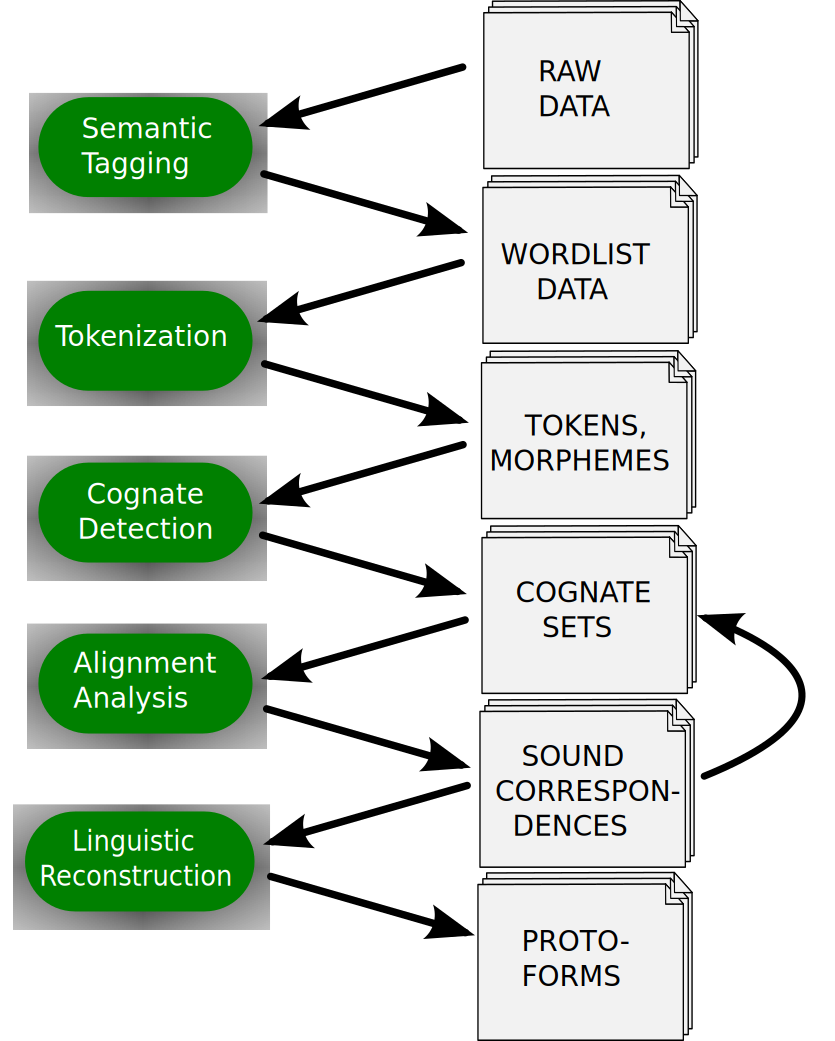
\includegraphics{img/workflow_basic.svg}}
& Dieser Workflow kann als allgemeines Konstrukt der von rohen Daten bis
hin zu Rekonstruktionen führt, angesehen werden. Nicht alle Schritte
können derzeit schon automatisch ausgeführt werden. Wir beschränken uns
daher auf die Schritte, die von den Wortlist-Daten hin zu den
Alinierungen führen.\tabularnewline
\bottomrule
\end{longtable}

\subsection{\texorpdfstring{{Workflows}}{Workflows}}

\subsubsection{\texorpdfstring{{Kognatenerkennung mit
LingPy}}{Kognatenerkennung mit LingPy}}

\textbf{Daten}

Wir nehmen einen Datensatz zu den chinesischen Dialekten, der als
TSV-Datei im LingPy Format vorliegt (File
"\href{https://github.com/LinguList/pyjs-seminar/blob/master/website/code/data/chinese.tsv}{chinese.tsv}").

Die Datei enthält neben den tabularen Daten auch eine JSON-Spezifikation
(eine Formaterweiterung in LingPy, die es erlaubt, JSON-Daten mit
einzubinden. Wir ignorieren diese Daten jedoch in diesem Zusammenhang.

\subsection{\texorpdfstring{{Workflows}}{Workflows}}

\subsubsection{\texorpdfstring{{Kognatenerkennung mit
LingPy}}{Kognatenerkennung mit LingPy}}

\textbf{Der Workflow}

Der Workflow gliedert sich in drei Schritte:

\begin{itemize}
\itemsep1pt\parskip0pt\parsep0pt
\item
  Kognatenberechnung:

  \begin{itemize}
  \itemsep1pt\parskip0pt\parsep0pt
  \item
    Einlesen der Datei in LingPy (LexStat Modul)
  \item
    Berechnen von Kognatensets mit Hilfe von LexStat
  \item
    Auslesen der Datei mit den neu berechneten Daten in TSV-Format
  \end{itemize}
\item
  Berechnen und Plotten eines phylogenetischen Baums
\item
  Berechnung der Alinierungen

  \begin{itemize}
  \itemsep1pt\parskip0pt\parsep0pt
  \item
    Einlesen der Datei in LingPy (Alignments Modul)
  \item
    Berechnen der Alinierungen mit Hilfe von Alignments
  \item
    Auslesen der Datei in HTML-Format
  \end{itemize}
\end{itemize}

\subsection{\texorpdfstring{{Workflows}}{Workflows}}

\subsubsection{\texorpdfstring{{Kognatenerkennung mit
LingPy}}{Kognatenerkennung mit LingPy}}

\textbf{Der Code}

\begin{verbatim}
from lingpy import *
# Schritt 1
## 1.1 Einlesen der Daten
lex = LexStat('data/chinese.tsv')
## 1.2 Kognatenerkennung
lex.cluster(method='sca', threshold=0.4)
## 1.3 Auslesen der Daten
lex.output('tsv', filename='data/chinese_lexstat', ignore='all')
# Schritt 2
## 1.1 Berechnen des Baums
lex.calculate('tree', ref="scaid") # scaid sind die automatischen kognaten
## 1.2 Plotten des Baums
from lingpy.convert.plot import plot_tree
plot_tree(lex.tree, degree=160, filename="data/chinese_tree", fileformat="svg")
## 1.3 Schreiben der Distanz-Daten
lex.output('dst', filename="data/chinese_distances")
# Schritt 3
## 1.1 Einlesen der Daten
alm = Alignments('data/chinese_lexstat.tsv', ref="scaid")
## 1.2 Alinierung
alm.align()
## 1.3 Auslesen der Daten in HTML
alm.output('html', filename='data/chinese_alignments')
\end{verbatim}

\subsection{\texorpdfstring{{Workflows}}{Workflows}}

\subsubsection{\texorpdfstring{{Kognatenerkennung mit
LingPy}}{Kognatenerkennung mit LingPy}}

\textbf{Die Ergebnisse: Der Baum}

\href{../code/data/chinese_tree.svg}{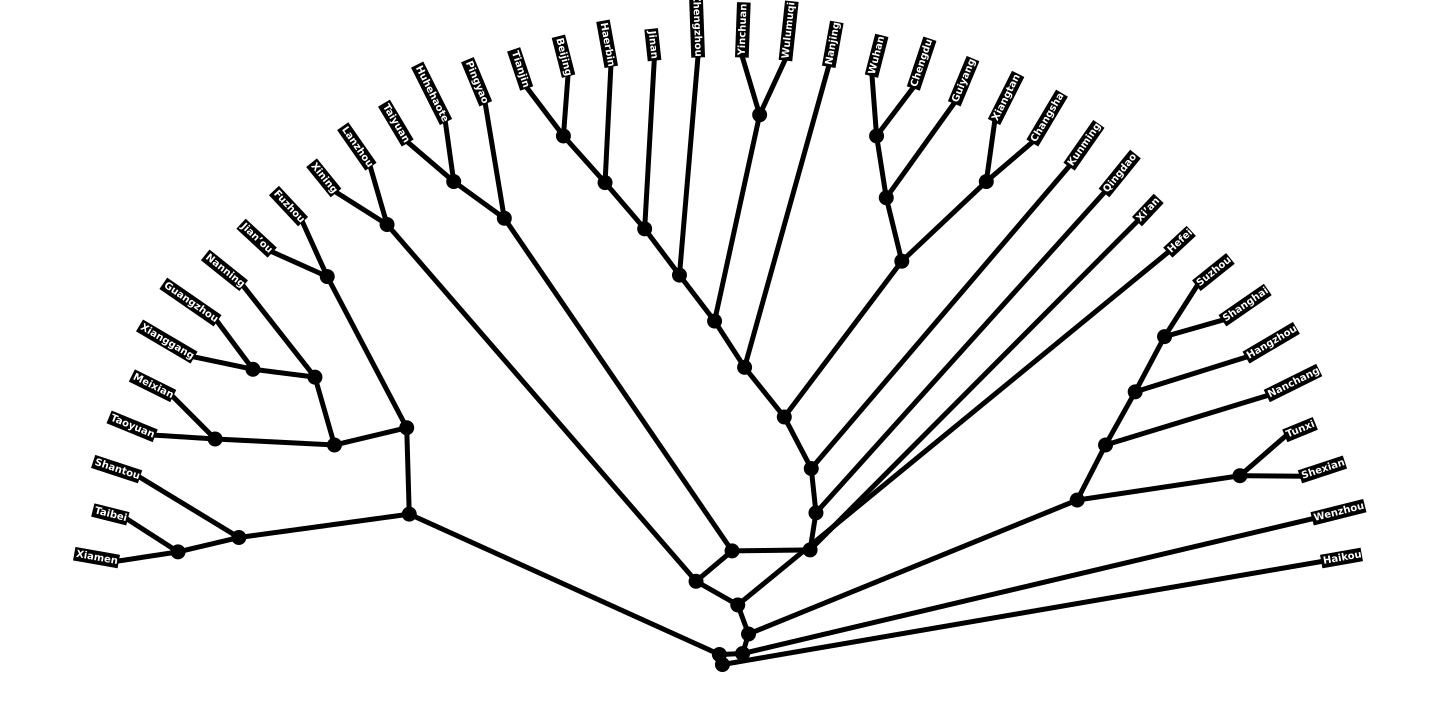
\includegraphics{../code/data/chinese_tree.svg}}

\subsection{\texorpdfstring{{Workflows}}{Workflows}}

\subsubsection{\texorpdfstring{{Kognatenerkennung mit
LingPy}}{Kognatenerkennung mit LingPy}}

\textbf{Die Ergebnisse: Die Alinierungen}

\subsection{\texorpdfstring{{Workflows}}{Workflows}}

\subsubsection{\texorpdfstring{{Integration mit externen
Tools}}{Integration mit externen Tools}}

\textbf{Einlesen der Daten in Splitstree}

Mit \href{http://splitstree.org}{SplitsTree} können wir Netzwerke aus
Distanzmatrizzen berechnen. Da wir die Distanzmatrix ja bereits
exportiert haben, genügt es, wenn SplitStree erfolgreich installiert
wurde, diese entweder direkt als Textdatei einzulesen, oder den Inhalt
der Datei
\href{ttps://github.com/LinguList/pyjs-seminar/blob/master/website/code/data/chinese_distances.dst}{chinese\_distances.dst}
zu kopieren und in den Editor von SplitsTree zu pasten.

\subsection{\texorpdfstring{{Workflows}}{Workflows}}

\subsubsection{\texorpdfstring{{Integration mit externen
Tools}}{Integration mit externen Tools}}

\textbf{Das Neighbor-Net der chinesischen Daten}

\href{../code/data/chinese_network.svg}{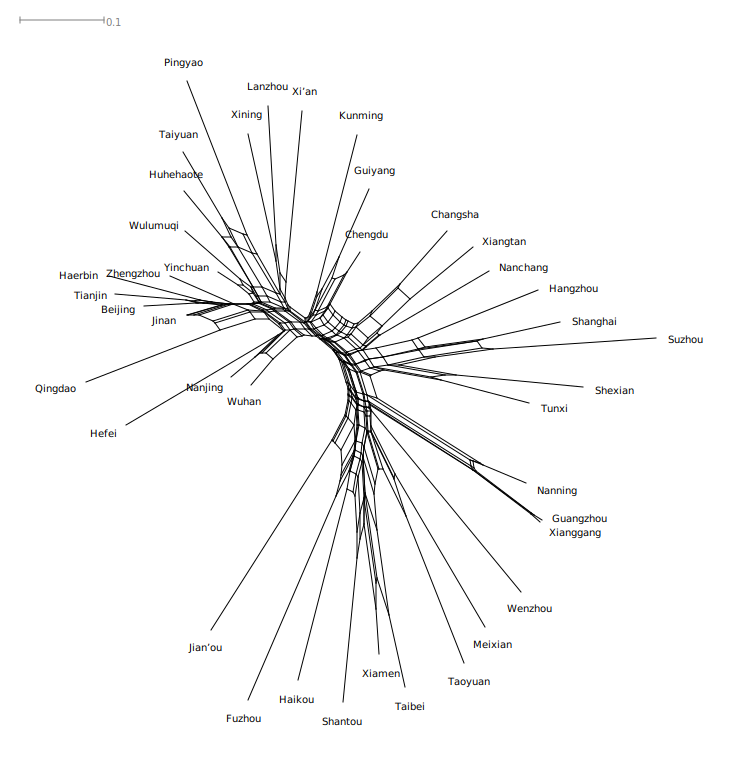
\includegraphics{../code/data/chinese_network.svg}}

\subsection{\texorpdfstring{{Agenda 2015}}{Agenda 2015}}

\begin{itemize}
\itemsep1pt\parskip0pt\parsep0pt
\item
  {Automatischer Sprachvergleich}

  \begin{itemize}
  \itemsep1pt\parskip0pt\parsep0pt
  \item
    {Sequenzdistanzen}
  \item
    {Kognatenerkennung}
  \item
    {Phylogenetische Rekonstruktion}
  \end{itemize}
\item
  {Sprachvergleich mit LingPy}

  \begin{itemize}
  \itemsep1pt\parskip0pt\parsep0pt
  \item
    {Eingabeformate}
  \item
    {Analysen}
  \item
    {Ausgabeformate}
  \end{itemize}
\item
  {Workflows}

  \begin{itemize}
  \itemsep1pt\parskip0pt\parsep0pt
  \item
    {Allgemeines vorweg}
  \item
    {Kognatenerkennung mit LingPy}
  \item
    {Integration mit externen Tools}
  \end{itemize}
\end{itemize}

\VERB|\NormalTok{>>> }\DecValTok{3} \NormalTok{- }\DecValTok{2}|

Ende der zweiten Sitzung

\href{../slides.html}{ÜBERBLICK}

\hyperdef{}{changeme}{}{\href{../slides.html}{Nächste Sitzung}}

\hyperdef{}{changeve}{}{\href{../slides.html}{Vorherige Sitzung}}

Vorherige Sitzung
